\documentclass{sigplanconf}

% Email drafts to: M. George Hansen, Evan Laforge, Ketil Malde, Sonke Hahn

\usepackage{amsmath}
\usepackage{amssymb}
\usepackage{natbib}
\usepackage{multirow}
\usepackage{setspace}
\usepackage{balance}
\usepackage[all]{xy}

\newcommand{\backticks}[1]{\mathsf{\text{\textit{\`{}}}#1\!\text{\textit{\`{}}}}\;}

\include{paper}
%include paper.fmt
%format (List (a) (b)) = "[" b "]_{" a "}"
%format (List_alpha b) = "[" b "]_{\alpha}"
%format Result_alpha = "\Varid{Result_\alpha}"
%format *> = "\mathbin{*\hspace{-5.8px}>}"
%format **> = "\mathbin{*\!*\hspace{-5.8px}>}"
%format *>> = "\mathbin{*\hspace{-5.8px}>\!\!>}"
%format ?> = "\mathbin{\raisebox{-.7px}{?}\hspace{-4px}>}"
%format ?== = "\mathbin{?\hspace{-4px}\equiv}"
%format `replaceExtension` = "\backticks{replaceExtension}"
%subst string a = "\!\text{\sf ``" a "\char34}\!"
%format context = "\Keyword{context}"
%format dependsS = "\Varid{depends\!^{*}}"
%format hashInclude = "\text{\sf ``\#include \textbackslash\char34\char34}"
%format Rule_m = "\Varid{Rule_m}"
%format Rule_s = "\Varid{Rule_s}"
%format build_m = "\Varid{build_m}"
%format build_s = "\Varid{build_s}"
%format Result_m = "\Varid{Result_m}"
%format Result_s = "\Varid{Result_s}"
%format skip_m = "\Varid{skip_m}"
%format skip_s = "\Varid{skip_s}"

\hsdef{\begin{comment}
alpha,r,self
IO,Main,Development.Shake
Any,Eq,Show,Hashable,NFData,MonadIO,TypeRep
contents
\end{comment}}

\begin{comment}
\h{.*}\begin{code}
import Data.Typeable
import Data.Hashable
import Control.DeepSeq
import Control.Monad.IO.Class
import Data.Monoid
import Control.Concurrent
import Data.Maybe
import Data.List hiding (find)
import Data.Binary
import Control.Monad
import System.Cmd
import System.Time
import qualified System.Directory
import System.Directory(copyFile,createDirectoryIfMissing)
data Map k v
data Set k
data Key
data Value
data Time = Time deriving (Ord,Eq)
type List_alpha a = [a]
hashInclude = "#include \""
ellipses = undefined
instance Binary ClockTime
instance NFData ClockTime
instance Eq Value
instance Typeable ClockTime
instance Hashable ClockTime
\end{code}
\h{.default}\begin{code}
instance Binary Dir
instance NFData Dir
instance Show Dir
instance Typeable Dir
instance Hashable Dir
instance Eq Dir
instance Binary File
instance NFData File
instance Show File
instance Typeable File
instance Hashable File
instance Eq File
instance Rule Files FileTimes
instance Binary Files
instance NFData Files
instance Show Files
instance Typeable Files
instance Hashable Files
instance Eq Files
instance Binary FileTimes
instance NFData FileTimes
instance Show FileTimes
instance Typeable FileTimes
instance Hashable FileTimes
instance Eq FileTimes
writeFileLines :: FilePath -> [String] -> Action ()
shakeVersion :: ShakeOptions -> Int
system' :: String -> [String] -> Action ()
readFileLines :: FilePath -> Action [String]
(*>>) :: [FilePattern] -> ([FilePath] -> Action ()) -> Rules ()
writeFile' :: FilePath -> String -> Action ()
writeFileChanged :: FilePath -> String -> Action ()
cIncludes :: FilePath -> IO [FilePath]
systemOutput :: FilePath -> [String] -> Action (String, String)
\end{code}
\h{.m}\begin{code}
(!) :: Set Rule_m -> Key -> Rule_m
data Rule
\end{code}
\h{.s}\begin{code}
(!) :: Set Rule_s -> Key -> Rule_s
\end{code}
\h{.s2}\begin{code}
instance Eq (Result_s -> Time)
instance Ord (Result_s -> Time)
\end{code}
\end{comment}


\newcommand{\file}{\textsf}
\newcommand{\prog}{\texttt}
\newcommand{\make}{\prog{make}}

\begin{document}
\conferenceinfo{ICFP'12,} {September 10--12, 2012, Copenhagen, Denmark.}
\CopyrightYear{2012}
\copyrightdata{978-1-60558-794-3/10/09}

\preprintfooter{}   % 'preprint' option specified.

\title{A Better Build System}
% \subtitle{}

\authorinfo{Neil Mitchell}
           {\verb"ndmitchell@gmail.com"}

\maketitle

\begin{comment}
1. State the problem
2. Say why it�s an interesting problem
3. Say what your solution achieves
4. Say what follows from your solution
\end{comment}

\begin{abstract}
Most complex software projects are compiled using a build tool (e.g. \make{}), which runs commands in an order satisfying user-defined dependencies. Unfortunately, most build tools require all dependencies to be specified \textit{before} the build starts. This restriction makes many common dependency patterns difficult to express, especially those involving files generated at build time. We show how to eliminate this restriction, allowing additional dependencies to be specified while building. We have implemented our ideas in the Haskell library Shake, which has been used for the last three years in a complex build system compiling millions of lines of code.
\end{abstract}

\category{D.3}{Software}{Programming Languages}

\terms
Languages

\keywords
build-system, compilation, Haskell

\section{Introduction}
\label{sec:introduction}

A build tool, such as \make{} \cite{make}, takes a set of build rules, plus some input files, and produces some output files. Using \make{}, a build rule can be written as:

\ignore\begin{code}
{-"\textsf{result.tar : file1 file2}"-}
    {-"\textsf{tar -cf result.tar file1 file2}"-}
\end{code}

\noindent This rule says that the file \file{result.tar} depends on the inputs \file{file1} and \file{file2} (first line), and provides a command to build \file{result.tar} (second line). Whenever \file{file1} or \file{file2} change, the command will be run, and \file{result.tar} will be built.

But imagine we want to build \file{result.tar} from the list of files stored in \file{list.txt}. The dependencies of \file{result.tar} cannot be specified in advance, but depend on \textit{the contents} of \file{list.txt}. Unfortunately, \make{} offers no easy way to express dependency (there are workarounds, but none are pleasant or effective). Using the build tool we develop in this paper, we can write:

\h{expr}\begin{code}
"result.tar" *> \_ -> do
    need ["list.txt"]
    contents <- readFileLines "list.txt"
    need contents
    system' "tar" $ ["-cf","result.tar"] ++ contents
\end{code}

This rule describes how to build \file{result.tar}. We depend on (|need|) the file \file{list.txt}. We read each line from \file{list.txt} into the variable |contents| -- being a list of the files that should go into \file{result.tar}. Next, we depend on all the files in |contents|, and finally call the \prog{tar} program. If either \file{list.txt} changes, or any of the files listed by \file{list.txt} change, then \file{result.tar} will be rebuilt.

The key difference from \make{} (and nearly all other build tools) is that rather than specifying all dependencies \textit{in advance}, we allow further dependencies to be specified \textit{after} examining the results of previous dependencies. This difference is crucial to accurately describe many dependency relationships.

Consider the problem of dependencies stemming from files included by a C source file. Many build tools require these dependencies to be specified manually. Some build tools can use two separate stages, where dependencies are computed (by scanning the files) and then built. But if the build system generates files and then compiles them, even a two stage system is insufficient, as the generated files are not available during the first phase. Our build tool has no such limitations -- it is able to easily handle generated files, even generated files which are only necessary due to being included by other generated files.

\subsection{Contributions}

We have implemented our build tool as a Haskell library, named Shake, which is available online\footnote{\url{http://hackage.haskell.org/package/shake}}. Shake provides a concise syntax for writing build systems (\S\ref{sec:user_view}), along with a high-performance implementation (\S\ref{sec:developer_view}). By implementing Shake as a Haskell library we allow rules to be written using the full power of Haskell, including the use of modules and functions to properly structure large build systems.

In addition to more flexible dependencies (\S\ref{sec:theory}), Shake also includes the important features of \make{}, such as minimal rebuilds (running only a subset of the rules when some subset of the inputs change, \S\ref{sec:cached_shake}), and parallelising the build (running multiple independent rules at the same time, \S\ref{sec:parallelism}). We allow rules to operate over arbitrary values, not limited to files, allowing us to properly handle rules producing multiple results (\S\ref{sec:multiple_outputs}). We have built a number of useful tools into Shake, including profiling (\S\ref{sec:profiling}) and dependency analysis (\S\ref{sec:analysis}).
 
% and build rule checking (\S\ref{sec:lint}).

Shake has been used at Standard Chartered for the past three years (\S\ref{sec:evaluation}). The build system creates over 30,000 build objects, with more than a million lines of source code and a million lines of generated code, in many programming languages. We originally implemented this build system using \make{}, but the result was slow to run, hard to maintain, and frequently caused spurious compile failures. Switching to Shake made our build system ten times shorter, made builds run twice as fast, and has solved our build system problems.

\section{Specifying Dependencies}
\label{sec:theory}

Most \make{}-like build tools start by constructing a graph from the dependency information, then traverse the graph, running the rules to build the required results (or use a topological sort, giving a similar effect). However, any approach based on a static dependency graph cannot permit additional dependencies to be specified while running the rules. As we saw in \S\ref{sec:introduction}, many examples \textit{require} additional dependencies to be specified while running rules. The solution is simple -- we reject the idea that build tools should use a static dependency graph.
In this section we model the dependencies used in non-recursive \make{}, as described by \citet{miller:recursive_make}, along with our enhanced dependency scheme. We describe what it means for a build system to be correct, and how to support minimal rebuilds. In \S\ref{sec:user_view} and \S\ref{sec:developer_view} we show how to turn these ideas into a usable tool.

\subsection{Moving Dependency Specification}

While the \make{} tool is heavily IO and file based, that is not an essential property of \make{}. To model dependency information, we use the type |Key| for things that can be created or are dependencies (i.e. file names), and the type |Value| for the values associated with a |Key| (i.e.  file contents). With these types, we can define our main |build| function as:

\h{.m}\begin{code}
build :: Set Rule -> Key -> Value
\end{code}

The |build| function takes a (possibly infinite) set of rules and the target |Key| to build, and returns the |Value| associated with that |Key|. We restrict our model to building only one target, while \make{} allows multiple targets (i.e. a list of |Key|s to build). However, we can encode multiple targets by creating a distinguished rule that depends on all the targets and returns all their values, and then make that single rule the target.

Using |build|, we can model \make{} by defining the |Rule| type as:

\h{.m}\begin{code}
data  Rule_m = Rule_m
      {  creates  :: Key
      ,  depends  :: [Key]
      ,  action   :: [Value] -> Value
      }
\end{code}

A \make{} |Rule| (|Rule_m|) can be modelled as the |Key| it |creates|, the |Key|s it |depends| on, and the |action| that takes the depended upon |Value|s and produces the result |Value|. Note that all dependencies for a rule are specified \textit{before} running the action.

Using the same |build| function, we can model our enhanced dependency scheme as:

\h{.s .s2}\begin{code}
data  Rule_s = Rule_s
      {  creates  :: Key
      ,  action   :: Action
      }

data Action  =  Depends Key (Value -> Action)
             |  Result Value
\end{code}

A Shake |Rule| (|Rule_s|) can be modelled as the |Key| it |creates|, and the |action| that creates the result. The |Action| either returns the |Result| |Value|, or requires a new dependency with |Depends| -- specifying the |Key| it depends on, plus a function that takes the |Value| of that |Key| and provides a new |Action|.

The big difference is the introduction of dynamic dependencies. A rule can dynamically, based on the values of previous dependencies, require additional dependencies. We can easily translate |Rule_m| to |Rule_s|, but the reverse is not possible -- |Rule_s| is strictly more powerful than |Rule_m|.

\subsection{Correctness}

Assuming a function named |(!)| which finds a |Rule| for a given |Key|, we can write a function to build |Rule_m| targets as follows:

\h{.m}\begin{code}
build_m rules target = run (rules ! target)
    where run r = action r (map (build_m rules) (depends r))
\end{code}

Starting at the |target| |Key|, we find the associated |Rule_m|, run |build_m| on its dependencies, and then run the |action|. A |Rule_m| build system is correct for a given target and set of rules iff the |build_m| function is total. If we assume all |action|s are total, then |build_m| is total if you can build a finite dependency graph for the target. This property can be checked without running any actions.

We can write a similar function to build |Rule_s| targets as follows:

\h{.s}\begin{code}
build_s rules target = run (action (rules ! target))
    where  run (Result val) = val
           run (Depends dep act) = run (act (build_s rules dep))
\end{code}

Starting at the |target| |Key|, we find the |action| from the associated |Rule_s|, and run it. If we encounter a |Result| we are done; if we encounter a |Depends| we run |build_m| on that dependency before continuing. As before, a |Rule_s| build system is correct for a given target and set of rules iff the |build_s| function is total. However, unlike before, there is no obvious way to predict termination in advance without detailed information about the |action| functions.

\subsection{Minimal Rebuilds}
\label{sec:minimal_rebuilds}

One important property of build tools is performing minimal rebuilds, something we ignored in the the previous section. In an execution of |build|, any action should be run at most once -- a property that is easy to ensure with a simple cache. Additionally, if an action has the same inputs as the last time it was run, it should not be repeated. In this section we first explore how to avoid repeating actions whose inputs have not changed with |Rule_m|, enhancing the scheme followed by \make{}, and then apply the same ideas to |Rule_s|.

\subsubsection{Minimal Rebuilds with |Rule_m|}
\label{sec:cached_make}

To avoid repeating actions whose inputs have not changed, \make{} does not run any actions where the input files have older modification times than the result file. We can use a similar scheme, adapted to work on arbitrary |Key|/|Value| types. Whenever an |action| is run, we create a |Result|:

\h{.m}\begin{code}
data Result_m = Result_m
    {  created  :: Key
    ,  result   :: Value
    ,  built    :: Time
    }
\end{code}

|Result_m| contains the |Key| the action |created|, the |result| |Value|, and the time when the result was |built|. We store all |Result_m| values between build runs, and skip rerunning a |Rule_m| if: 1) the |creates| |Key| has a result available; 2) all the |depends| |Key|s have results available; and 3) the |built| field of the result associated with |creates| is greater than or equal to all the |built| fields of the results associated with |depends|. Given a function named |ask| to lookup the associated result for a |Key|, which returns |Nothing| if the there is no associated result, we can write:

\h{.m}\begin{code}
skip_m :: (Key -> Maybe Result_m) -> Rule_m -> Bool
skip_m ask r  |  Just self  <- ask (creates r)
              ,  Just deps  <- mapM ask (depends r)
              =  all ((<= built self) . built) deps
\end{code}

The |skip_m| function returns |True| if a rules action does not need running. We first check that there is a |Result_m| associated with the |creates| of this rule, then that every |depends| has a result (using the |mapM| to require every |ask| call returns |Just|), then check that all dependencies were build before this action was run.

The \make{} approach of relying on the system time can fail if the system clock changes, or if a file is modified but has its value set to an older timestamp -- such as when extracting a backup which resets the timestamp. Therefore, instead of using the system time for |built|, we use the number of runs of this build system, and increment |Time| each run, guaranteeing that |Time| is monotonically increasing.

A convenient property of the \make{} approach is that no additional data need be stored between runs, since the file system already stores modification times. In contrast, we must store the |Time| and |Result_m| values in some persistent data store (an additional data store is required for many advanced build systems, see \S\ref{sec:related_work}). However, for some types of rules, such as when |Value|s are filenames and |Key|s are modification times, we end with the |Value|s stored in both the data store \textit{and} the file system (or another persistent store). If an inconsistency is detected, we must remove our stored result. We can detect inconsistencies given the following function:

\begin{code}
validStored :: Key -> Value -> Bool
\end{code}

This function should return |True| when the |Key|/|Value| are not stored elsewhere, or when they are stored but the |Value| is consistent. As an example, for files |validStored| should return |True| only if the file exists, and has the same modification time.

\subsubsection{Minimal Rebuilds with |Rule_s|}
\label{sec:cached_shake}

To achieve minimal rebuilds with |Rule_m| we rely on having the dependencies available without executing the action, something that is not available with |Rule_s|. To solve this problem, we include the list of dependencies in |Result_s|, and use them in |skip_s|:

\h{.s}\begin{code}
data Result_s = Result_s
    {  created  :: Key
    ,  result   :: Value
    ,  built    :: Time
    ,  depends  :: [Key]
    }

skip_s ask r  |  Just self  <- ask (creates r)
              ,  Just deps  <- mapM ask (depends self)
              =  all ((<= built self) . built) deps
\end{code}

Compared to |skip_m|, we have made one change -- instead of using \h{.s}|depends r|, we use \h{.s}|depends self|. With this modification we are able to ensure minimal rebuilds using |Rule_s|. We still require the |validStored| check from the previous section.

\subsubsection{Unchanging Results}
\label{sec:unchanging_results}

The \make{} tool has a requirement that a rule action \textit{must} modify the file it creates, otherwise the rule will be repeatedly rerun, as the result will remain older than its dependencies. However, since we are storing |built| separately from |result|, we can do better, eliminating some unnecessary rebuilds.

Instead of storing just the |built| time, we also store the |changed| time -- when the |result| last changed. Whenever we create a result we use the current time for |built|, but if the |result| |Value| is the same as last time, we leave its |changed| time the same. We can rewrite |skip_s| to take advantage of this additional information:

\h{.s2}\begin{code}
data Result_s = Result_s
    {  created  :: Key
    ,  result   :: Value
    ,  built    :: Time
    ,  depends  :: [Key]
    ,  changed  :: Time
    }

skip_s ask r  |  Just self  <- ask (creates r)
              ,  Just deps  <- mapM ask (depends self)
              =  all ((<= built self) . changed) deps
\end{code}

We have only changed the final line of |skip_s| -- instead of checking against the |built| time of the dependencies, we check against the |changed| time. Since it is always the case that \h{.s2}|changed <= built|, |skip_s| will now return |True| more often.

For certain practical examples, support for unchanging results can reduce rebuild times from many minutes to seconds. As an example, consider a generated source file. If the generator changes it is necessary to regenerate the file, but there is a chance the result will be the same. By supporting unchanging files we can avoid rebuilding everything depending on that generated file.

\section{Shake in Haskell}
\label{sec:user_view}

In this section we go from the theory of \S\ref{sec:theory} to a practical build tool, structured as a Haskell library. In particular, we describe how to replace |Key| and |Value| with standard polymorphism, how to integrate IO into the actions and how to define the set of rules. We present the interface to Shake, but leave most implementation concerns to \S\ref{sec:developer_view}.

\subsection{A Shake Example}
\label{sec:c_example}

\begin{figure}
\begin{code}
{-"\Keyword{import}\;\Conid{Development.Shake}"-}
import System.FilePath

main = shake shakeOptions $ do
    want ["Main"]

    "Main" *> \out -> do
        cs <- getDirectoryFiles "." "*.c"
        let os = map (`replaceExtension` "o") cs
        need os
        system' "gcc" $ ["-o",out] ++ os

    "*.o" *> \out -> do
        let c = replaceExtension out "c"
        need [c]
        headers <- cIncludes c
        need headers
        system' "gcc" ["-o",out,"-c",c]

cIncludes :: FilePath -> Action [FilePath]
cIncludes x = do
    (stdout,_) <- systemOutput "gcc" ["-MM",x]
    return $ drop 2 $ words stdout
\end{code}
\caption{A Shake build system for C code.}
\label{fig:demo}
\end{figure}

Figure \ref{fig:demo} shows an example build system in Shake. Running this program will build \file{Main} from all the \file{*.c} files in the current directory. If we add or remove a \file{.c} file, or change any of the \file{.c} files or the header files they @#include@, then the necessary files will be recompiled.

The build system produces (|want|s) the file \file{Main}. To generate \file{Main} we list all the C files in the current directory, change their extensions to \file{.o} (object files), require those files to be built (|need| them), then call \prog{gcc} to link them. To build an object file we take the associated C file and call the function |cIncludes| to get the headers it requires. We |need| those headers, then call \prog{gcc} to do the compilation. The |cIncludes| function works by calling \prog{gcc -MM}, causing \prog{gcc} to generate the dependency information to the standard output.

This example demonstrates a number of features of Shake based build systems:

\begin{description}
\item[It's Haskell] The |main| entry point can call |shake| directly, but it can also do command line processing (\S\ref{sec:command_line}), or anything else. We have defined a local function, |cIncludes|, helping to split the build system into components that could be reused. We make use of the existing filepath library.
\item[Accurate dependencies] The call to |getDirectoryFiles| is tracked (\S\ref{sec:directory_rule}) -- if the results change, it will trigger a rebuild. We also track the dependencies introduced by @#include@ directives.
\item[We use system commands] We use \prog{gcc} to compile, to link, and to determine the headers required by the C files. We can freely use both Haskell functions and system commands to generate build results.
\end{description}

\subsection{Core Shake}
\label{sec:core_shake}

\begin{figure}
\begin{code}
data  ShakeOptions = ShakeOptions
      {  shakeFiles :: FilePath
      ,  shakeThreads :: Int
      {-" ,  \ldots"-}
      }

shakeOptions = ellipses -- default set of options

data Rules alpha
instance Monad Rules
instance Monoid alpha => Monoid (Rules alpha)

data Action alpha
instance Monad Action
instance MonadIO Action

class (
    Show key, Show value,
    Typeable key, Typeable value,
    Hashable key, Hashable value,
    Eq key, Eq value,
    Binary key, Binary value,
    NFData key, NFData value
    ) => Rule key value | key -> value where
    validStored :: key -> value -> IO Bool
    validStored k v = return True

run :: ShakeOptions -> Rules () -> IO ()

action :: Action a -> Rules ()

rule, defaultRule :: Rule key value =>
    (key -> Maybe (Action value)) -> Rules ()

apply :: Rule key value => [key] -> Action [value]
apply1 :: Rule key value => key -> Action value
\end{code}
\caption{Primitive operations in Shake}
\label{fig:shake_core}
\end{figure}

The primitive interface to Shake is given in Figure \ref{fig:shake_core} -- everything else is defined on top. At its essence, a Shake build system is a set of rules. We can run the rules with |run|, create new rules with |rule|/|defaultRule|, and when defining a rule we can express dependencies with |apply|/|apply1|.

We execute a set of rules with the |run| function, which also takes an options record. Typical options include which file to store the cached versions in (|shakeFiles|), and the number of processors to use (|shakeThreads|). These options are also used to select which mode to run Shake in, as described in \S\ref{sec:tools}.

Every rule that is defined or applied in Shake must be a member of the |Rule| class. The |Rule| class defines the method |validStored| to determine whether a value is consistent with the value stored externally. We require that each rule |key| has only one associated type of |value| -- a restriction that is not strictly necessary, but forces users to keep their rules simple. Each |key|/|value| type must also be a member of several type classes:

\begin{description}
\item [Typeable] We allow multiple types of rules in a single build system. To distinguish the types, we require a |Typeable| constraint, allowing us to obtain an explicit |TypeRep| \cite{lammel:syb}.
\item [Eq] We require equality to test if values are equal.
\item [Binary] We require |Binary| to store the values in a database, to achieve minimal rebuilds (\S\ref{sec:minimal_rebuilds}).
\item [Hashable] We require |Hashable| to lookup entries quickly.
\item [Show] We require |Show| for debugging messages and logging (\S\ref{sec:profiling}).
\item [NFData] We require |NFData| to ensure that values are fully evaluated when they are computed, ensuring that errors occur in a timely manner (\S\ref{sec:handling_errors}).
\end{description}

Normal rules are defined with |rule|, which requires a function which takes a single |key| value, and returns |Nothing| to indicate that this rule does not build this |key|, or |Just| with the action necessary to build the associated |value|. If two rules match the same key then an error is raised. The function |defaultRule| allows a rule to be defined with a lower priority, which is used if no normal rules match -- for an example see \S\ref{sec:file_rules}. Instead of defining targets to build, we allow actions to be specified using |action|, which are always run. The |Rules| type is a |Monoid|, allowing two sets of rules to be appended to produce a new set of |Rules|. In practice, the syntactic sugar supported by |Monad| is often a more natural way to define many rules, so we also make |Rules| a |Monad|. The |Action| type is a |Monad| and has an instance for |MonadIO|, allowing users to call arbitrary |IO| functions using |liftIO| to translate \h{type}|IO alpha| to \h{type}|Action alpha|.

The |apply1| function takes a |key|, ensures the |key| is built, and returns the associated |value|. The |apply| function can be thought of as |mapM apply1|, but is defined to build all necessary dependencies in parallel (see \S\ref{sec:parallelism}).

We have deliberately kept the core of Shake small, defining all specific types of rule outside. We describe how to implement this core in \S\ref{sec:developer_view}.

\subsection{Wildcard File Patterns}
\label{sec:file_pattern}

The \make{} tool supports the syntax \textsf{\%.c} to match any files ending with \file{.c}. We define a similar notation, allowing |"*"| to match any part of a filename, and |"//"| to match any number of directories, using the definitions:

\begin{code}
type FilePattern = String
(?==) :: FilePattern -> FilePath -> Bool
\end{code}

As an example, |"*.c" ?== "foo.c"| returns |True|, while |"*.c" ?== "foo.h"| returns |False|. We reuse the |FilePattern| type in several of our rules.

\subsection{Defining Rule Types}
\label{sec:directory_rule}

\begin{figure}
\begin{code}
import qualified System.Directory as IO

data Dir = Dir FilePath FilePattern
-- plus all necessary instances

go :: Dir -> IO [FilePath]
go (Dir dir pat) =
    liftM (filter (pat ?==)) $ IO.getDirectoryContents dir

instance Rule Dir [FilePath] where
    validStored q a = liftM (== a) $ go q

getDirectoryFiles :: FilePath -> FilePattern -> Action [FilePath]
getDirectoryFiles dir pat = apply1 $ Dir dir pat

defaultDir :: Rules ()
defaultDir = defaultRule $ Just . liftIO . go
\end{code}
\caption{Implementation of |getDirectoryFiles|.}
\label{fig:getdirectoryfiles}
\end{figure}

A typical Shake build system will use a handful of different |key|/|value| types. To aid end users, we suggest that people defining rule types also define sugar functions, as we have done for the rule types included with Shake. As an example of defining a rule type, we give the code for |getDirectoryFiles| in Figure \ref{fig:getdirectoryfiles}. This function takes a directory, and a file pattern (\S\ref{sec:file_pattern}), and returns the list of files that match.

We start by defining a |key| data type (|Dir|), along with a function that computes the result (|go|). We define a |Rule| instance mapping from the |Dir| data type to the result type of \h{type}|[FilePath]|, which uses equality to check if a previous result is still valid. We define |getDirectoryFiles| as a strongly typed wrapper around |apply1|, and |defaultDir| as a wrapper around |defaultRule|. Anyone wishing to use |getDirectoryFiles| should include |defaultDir| in their rule set. We do not export the |Dir| constructor, so users are force to use the wrappers.

\subsection{File Based Rules}
\label{sec:file_rules}

\begin{figure}
\begin{code}
import qualified System.Directory as IO

newtype File = File FilePath
-- plus all necessary instances

getFileTime :: FilePath -> IO (Maybe ClockTime)
getFileTime x = do
    b <- IO.doesFileExist x
    if not b then return Nothing else do
        liftM Just $ IO.getModificationTime x

instance Rule File ClockTime where
    validStored (File x) t = fmap (== Just t) $ getFileTime x

need :: [FilePath] -> Action ()
need xs = (apply $ map File xs :: Action [ClockTime]) >> return ()

defaultFile :: Rules ()
defaultFile = defaultRule $ \(File x) -> Just $ do
    res <- liftIO $ getFileTime x
    let msg = "Error, file does not exist and no rule: " ++ x
    return $ fromMaybe (error msg) res

want :: [FilePath] -> Rules ()
want xs = action $ need xs

(?>) :: (FilePath -> Bool) -> (FilePath -> Action ()) -> Rules ()
(?>) test act = rule $ \(File x) ->
    if not $ test x then Nothing else Just $ do
        liftIO $ createDirectoryIfMissing True $ takeDirectory x
        act x
        res <- liftIO $ getFileTime x
        let msg = "Error, rule failed to build the file: " ++ x
        return $ fromMaybe (error msg) res

(**>) :: [FilePattern] -> (FilePath -> Action ()) -> Rules ()
(**>) test act = (\x -> any (?== x) test) ?> act

(*>) :: FilePattern -> (FilePath -> Action ()) -> Rules ()
(*>) test act = (test ?==) ?> act
\end{code}
\caption{Implement of file rules.}
\label{fig:file_rules}
\end{figure}

While our build system is not restricted to rules dealing with files, in practice many build systems are file orientated. When implementing file rules, the filename is an obvious |key|, but |value| could equally be modification time or a hash of the file contents (e.g. SHA1). In practice, we found that using modification time is faster (significantly faster for large files) and being able to force rebuilds with \prog{touch} is highly convenient. Of course, our design allows anyone to define a new file rule, based on file content hashes.

We define file rules in Figure \ref{fig:file_rules}. To force files to be built, we define |need| and |want|. The |need| action demands all the modification times associated with the filenames, then throws away the result -- a computation depends on the time a file was built, but rarely uses the modification time in its computation. We define |want| as simply a |need| run as an action.

We define |defaultFile| as a rule that checks if the file is already present, and if so uses it. Source files will have no associated rules to build them, so this rule just records their modification time. If a file has no rules (since any rules would be run in preference to the default rule), and does not exist, we give an error to the user. As with |defaultDir|, anyone using |want|/|need| should include |defaultFile| in their rule set.

We define new file rules with |(?>)|, which takes a predicate to match against the file name and an action to run. This function forces the correct types, and obtains the modification time afterwards. Before running the action we create the directory containing the output file, an idea taken from the Ninja build system \cite{ninja}. We found that when running a large set of newly written rules, often one rule would create the output directory while another did not -- meaning some rule orderings worked while others failed. Automatically creating the output directory removes this source of failure.

While |(?>)| is the ultimate file creation rule, we define two additional operators, in terms of a wildcard match operator |(?==)| (\S\ref{sec:file_pattern}). We define |(*>)| for matching a single pattern, for example |"*.c" *> ellipses|, in a very similar manner to \make{}. We also define |(**>)| for matching any one of a set of patterns. In our large evaluation (\S\ref{sec:evaluation}), we found that |(?>)| was used about 5\% of the time, |(**>)| was used about 10\% and |(*>)| was used about 85\% of the time. In our experience, use of |(?>)| is a sign that the build system is poorly designed and should be rethought (our large evaluation used |(?>)| exclusively for compatibility with the system it replaced).

As a practical concern, when writing file rules, often there are multiple types of object that build \file{*.o} files. This problem can be easily solved by making Haskell produce \file{*.hs.o}, C produce \file{*.c.o} etc.


\subsection{Automatically Include Default Rules}
\label{sec:include_default_rules}

With the rule types already defined, users can write a build system using Shake. Unfortunately, if the user forgets to include the rule |defaultFile|, there is likely to be a runtime error. Instead of requiring the user to remember to include the default rules, we instead define a wrapper function |shake| which includes all the standard default rules:

\begin{code}
shake opts rules = run opts $ do
    defaultDir   -- \S\ref{sec:directory_rule}
    defaultFile  -- \S\ref{sec:file_rules}
    ellipses
    rules
\end{code}

In addition to the directory and file rules, we also include rules that query the existence of files, always force a rule to rerun, store arbitrary configuration data in a tracked manner and build multiple files in one action. All these rules are defined in a similar way to the directory and file rules.

The astute reader may be wondering why we can't move |defaultRule| into the |Rule| type class, and avoid requiring such a wrapper. Alas, that solution doesn't work because we need explicit rules of each type to deserialise dynamically typed values (for full details see \S\ref{sec:dynamically_typed}).

\subsection{Additional Functions}
\label{sec:derived}

Using the file rules (\S\ref{sec:file_rules}), we can safer versions of operations such as |readFile|/|copyFile|:

\begin{code}
readFile' :: FilePath -> Action String
readFile' x = need [x] >> liftIO (readFile x)

copyFile' :: FilePath -> FilePath -> Action ()
copyFile' old new = need [old] >> liftIO (copyFile old new)
\end{code}

These operations mirror their standard counterparts, but automatically include a |need| call. We also define a number of additional functions for working with files. The functions |readFileLines| and |writeFileLines| deal with files which should be treated as a list of lines. The function |writeFileChanged| writes a file, but only if the contents have changed, avoiding rebuilding by making use of unchanging results (\S\ref{sec:unchanging_results}).

We define the |system'| function which take a list of command line arguments, and escapes them as necessary, before calling the underlying |system| command. This function also contributes generates profiling information (see \S\ref{sec:profiling}). The |system'| function should be used carefully, as it cannot tell which files the system command may depend on, so explicit |need| commands must be used. We recommend writing wrappers around system commands which insert the appropriate |need| calls.

% (see \S\ref{sec:lint} for ways to detect such a problem)


\section{Implementing Shake}
\label{sec:developer_view}

We have implemented Shake, and used it extensively. In this section we sketch some of the main implementation challenges and how they can be overcome. We first describe how to implement multiple |key|/|value| types within a single build system, how to deal with errors, and finally how to execute the rules efficiently and with maximum parallelism. Readers interested in the full implementation are welcome to download the associated package (see \S\ref{sec:introduction}).

\subsection{Dynamically Typed Values}
\label{sec:dynamically_typed}

A single Shake program can use multiple types of keys and values. To work with heterogenous values in Haskell we define:

\ignore\begin{code}
data Any = Any (forall alpha bullet
    (  Typeable alpha, Eq alpha, Binary alpha
    ,  Hashable alpha, Show alpha, NFData alpha) => alpha)
\end{code}

This definition, using existentials \cite{laufer:existentials}, allows anything supporting all the type classes required to be stored with type |Any|. We can define |Key| and |Value| types in terms of |Any|. We can implement |Eq|, |Show|, |Hashable| and |NFData| instances for |Any| without difficulty, often by appealing to the |TypeRep| provided by the |Typeable| instance.

Implementing a |Binary| instance for |Any| is harder. Serialising a value is easy, but deserialising a value is problematic -- we can deserialise a |TypeRep|, but then we need to obtain the |get| method from the |Binary| instance associated with that type. The solution is to keep a table mapping |TypeRep|s to |Any| values containing the appropriate |Binary| instance. This table must include every type stored in the file we are reading, or it cannot be deserialised. We populate the table using all rules defined by |rule| and |defaultRule| in |Rules| -- which means we cannot move |defaultRule| into the |Rule| type class, as then a type could be usefully used without appearing in |Rules|, and would be missing from the table.

When deserialising, if we encounter a type not present in the table, we ignore the entire database. This is pessimistic, but safe -- if the set of types has changed that implies the build system has changed, which is not tracked anyway (see \S\ref{sec:changing_rules}).

\subsection{Handling Errors}
\label{sec:handling_errors}

To turn Shake into a practical system, we make a number of changes from the natural implementation, designed to improve errors handling.

\paragraph{Tracking the stack} We maintain a stack while executing rules, listing the keys that cause a rule to be executed. Whenever an error occurs, either when running a rule or trying to find a rule, we print the stack. Whenever we execution an action, we force its result using the |NFData| instance, ensuring any errors are raised with the correct stack. We raise an error when trying to build a key that is already on the stack, which would indicate a key depends on itself. This check allows us to give a clear error message where otherwise there would have been an infinite loop.

\paragraph{Tracing and diagnostics} We provide options to print every rule run, and every system command run. Whenever a system command fails, we reprint the command line after the failure, to ensure the command has not scrolled off the screen. We provide a diagnostics mode to print detailed information as the build progresses, helping to debug build systems.

\paragraph{Resuming after errors} When running a large build system, it is common for it to fail before completing -- either from a rule raising an error, or the end user killing the build process. In these cases it is important that none of the work that has been performed is lost -- therefore we maintain a journal and every time a rule finishes running we immediately store the result. If Shake completes successfully we delete the journal. If on restarting Shake has a journal file, we replay the journal.

\subsection{Build Algorithm}

The internal state of Shake includes a mapping from each key to one of six status values. At the start of a build run, every key is either |Loaded| (was found in the database) or |Missing| (is not known to the build system). The build logic of Shake is implemented in a function named |build|, which modifies the state to ensure that a given key is either |Ready| (a result is available) or |Error| (there was an exception when running the rule). The |build| function is parameterised by a way to check a stored value is valid (|validStored| from \S\ref{sec:core_shake}) and a way to build a key (appealing to the defined |rule|s for that type). Using |build|, it is relatively easy to implement the core of Shake -- simply run all |action|s and make |apply| call |build| before looking up the status of a key.

Our implementation of the |build| function takes 100 lines of Haskell. While implementing |build| there are two separate challenges, \textit{correctness} and \textit{efficiency}.

\subsubsection{Correctness}

\begin{figure}
\begin{center}
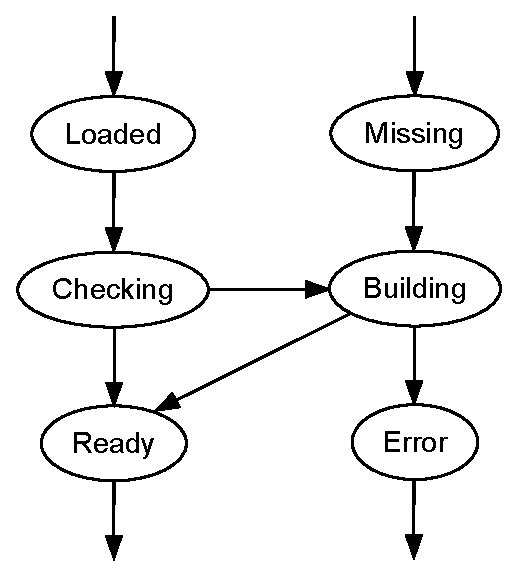
\includegraphics[scale=0.6]{states.eps}
\end{center}
\caption{Result states and transitions.}
\label{fig:states}
\end{figure}

For an implementation of |build| to be correct, it must always execute enough rules to ensure that the results are correct, but never execute rules that could have been safely skipped. We satisfy these constraints with the status transition diagram in Figure \ref{fig:states}. At the start of a build run all keys are either |Loaded| or |Missing|, and after calling |build| on a key, it is either |Result| or |Error|. We use |Checking| for keys that are being checked to see if they are correct or need rebuilding, and |Building| for rules that are currently being built. If a key is |Missing| and is demanded we have no choice but to start |Building| it. After |Building| a key, the action will either successfully produce a |Result|, or fail producing an |Error|.

Most of the complexity of |build| comes from the |Checking| state, in order to support unchanging results (\S\ref{sec:unchanging_results}). When checking a key there are two possibilities -- either the check succeeds and we have a correct |Result|, or the check fails and we transition to |Building|. We first check the stored result using |validStored|, failing if the result is no longer valid. We then |build| each dependency in order, and fail if the dependency is |Error|, or if it has changed since we built this key. If all dependencies are checked successfully, we transition to |Result|.

To check if a dependency has changed we may end up building the dependency before running the rule that requires it. As a result, if a key ends up in the |Error| state, the build may still complete successfully. If the build system has changed, and the new rule no longer requires its previous dependency, then running the rule afresh may succeed. To reduce the possibility of building many redundant keys, we always check the dependencies of a rule in the order they were required, ensuring that if the rules are deterministic and have not changed since the previous build, then all executed rules will be required.

\subsubsection{Efficiency}
\label{sec:parallelism}

When implementing |build| there are two separate efficiency goals. If no rules need to be run (a common case), |build| should strive for low overhead, as the time of |build| is likely to be a significant proportion of the total time. If rules do need running, |build| should try to start the rules as early as possible, to maximise parallelism. In order to expose parallelism we make |build| take a set of keys, and store |depends| as \h{type}|[[Key]]| instead of just \h{type}|[Key]| -- where each entry comes from one call to |apply|

In some ways the goals of low overhead and high parallelism are in conflict -- the first is best served by being single threaded (avoiding locks and thread contention), while the second suggests spawning many threads whenever we encounter a list of activities that could potentially be run in parallel. Our approach is to use a thread pool for running rules, and a single lock to protect the state (no fine-grained locking). The function |build| takes the state lock, and on a single thread, performs as many transitions as it can without blocking or running any rules. Any blocking is performed after the state lock has been released, and any rules are run by adding them to the thread pool and blocking on the result. By using a thread pool we obtain high levels of parallelism, and by having a single state lock we can perform a build with no rules with only a single lock and no threads.

Our thread pool obeys the |shakeThreads| flag (\S\ref{fig:shake_core}), ensuring no more than a given maximum number of rules are running at one time. The thread pool is based around a pool of workers. If a new task is added to the pool, and less than |shakeThreads| workers are active, a new thread is spawned, otherwise it is queued until a worker completes. When a rule is blocked in |build|, waiting for dependencies to build, we notify the thread pool to temporarily spawn another worker, ensuring maximum parallelism.

In order to reduce contention between processes, we run tasks added to the thread pool in a \textit{random} order. Often different operations in a build require different resources -- for example a compiler uses a lot of CPU while a linker does a lot of disk access. If we run tasks in the order they were added, certain dependency structures will run all compilers followed by all linkers, resulting in lots of resource contention between different processes. A random ordering avoids the worst case scenario, and gives a noticeable speedup -- up to 20\% for some real build systems.

\section{Evaluation}
\label{sec:evaluation}

% Our build system has a maximum of 20 levels deep of |apply| calls from the top-level |action| statement, but 80\% of build rules are between 3 and 7 steps deep.

% [(0,2127),(1,22651),(2,190623),(3,64795),(4,15666),(5,22732),(6,10583),(7,11801),(8,5658),(9,5035),(10,3144),(11,2500),(12,974),(13,605),(14,251),(15,230),(16,73),(17,25),(18,25),(19,6),(20,1)]

At Standard Chartered we have been using a build system based on Shake for three years. Before Shake we used \make{}, but \make{} was a poor fit for our project, primarily due to a large number of generated files. In common with many large projects, we were forced to split our build system into several phases, where one phase generated some files and \make{} rules which were used by a subsequent phase. Before we switched to Shake, we had over 10,000 lines of \make{} rules which were very brittle and hard to extend.

Our Shake based build system has been an unqualified success -- while the complexity of our project has increased (more files, more compilers, more generators and more platforms), the build system has coped well. The first version of our Shake build system was under 1000 lines and matched everything the \make{} system did. Shake has been able to express all the dependencies correctly and directly, resulting in a robust build system.

From experience implementing several build systems using Shake we have learnt a number of lessons -- both about best practices for structuring build systems, and how the underlying core of Shake can be used to deal with the complexities of real software. In this section we share some of those lessons.

\subsection{Command Line Interface}
\label{sec:command_line}

While the |shake| function can be used as |main|, it offers no support for command line arguments. We use the |shake| function to build a program \prog{mk}, which handles command line options, allowing us to specify some of the fields in |ShakeOptions| (Figure \ref{fig:shake_core}), such as parallelism and verbosity.

One essential feature of any build tool is the @clean@ command, which deletes all build objects. Using Shake we could query the database to find all build results, and delete them. Alternatively, deleting the database will cause a full rebuild. However, we have found the most convenient solution is to create all build objects in a folder \file{.make}, and clean our project by deleting that directory.

Using \make{}, you can specify build targets on the command line. We have implemented an enhanced version of this feature, allowing both individual files and sets of files to be enabled/disabled. As an example, a user may write @mk !DOCS@ to disable building documentation, or @mk index.html@ to build only \file{index.html}. We control these targets by passing a modified version of |want| to the functions specifying rules, which consults the command line arguments:

\begin{code}
documentation :: (String -> [FilePath] -> Rules()) -> Rules ()
documentation wants = do
    wants "DOCS" ["index.html"]
    "index.html" *> \out -> ellipses
\end{code}

\subsection{Multiple Outputs}
\label{sec:multiple_outputs}

Some programs, such as the Haskell compiler \prog{ghc} \cite{ghc7_2}, can produce two outputs from one action -- compiling \file{Foo.hs} produces both \file{Foo.o} and \file{Foo.hi}. As a first approximation, the \file{.o} file depends on the entire contents of the file, while the \file{.hi} file depends only on the type signatures. A single \prog{ghc} invocation needs to do all the work to produce both, but often the \file{.hi} file will be left unchanged. Unfortunately, many build systems (including \make{}) do not handle multiple outputs well.

In Shake, it is usually possible to fake multiple outputs with single file dependencies -- claiming that \file{Foo.hi} depends on \file{Foo.o} with no action and \file{Foo.o} depends on \file{Foo.hs} by running \prog{ghc}. Thanks to support for unchanging files (see \S\ref{sec:unchanging_results}), the \file{.hi} file will not cause a rebuild unless it changes. However, this rule has two problems:

\begin{itemize}
\item If \file{Foo.hi} is deleted \textit{without} also deleting \file{Foo.o}, then \file{Foo.hi} will not be rebuilt and the build system will be incorrect.
\item If \prog{ghc} updates \file{Foo.hi}, but manages to determine it does not need to update \file{Foo.o}, then \file{Foo.hi} will not be marked as dirty and the build will be incorrect.
\end{itemize}

Despite these limitations, the fake single file dependency is usually sufficient. However, consider a command that reads \file{numbers.txt} containing lines of numbers, and produces \file{even.txt} and \file{odd.txt} -- each containing only the even or odd numbers -- but does not update an output file that has not changed. In this situation there is no fake dependency that properly captures the flow of updates. Fortunately, we can capture the proper meaning by introducing a new type or rule, for rules which produce multiple files.

\begin{code}
data Files = Files [FilePath]
data FileTimes = FileTimes [ClockTime]

multipleOutputs = do
    rule $ \(Files xs) ->
        if xs /= ["even.txt","odd.txt"] then Nothing else Just $ do
            need ["numbers.txt"]
            system' "number-split" []
            times <- liftIO $ mapM getFileTime xs
            return $ FileTimes $ map fromJust times

    ["even.txt","odd.txt"] **> \_ -> do
        apply1 (Files ["even.txt","odd.txt"]) :: Action FileTimes
        return ()
\end{code}

Inside |multipleOutputs|, the call to |rule| declares a rule that can build both \file{even.txt} and \file{odd.txt} in a single step. We call the \prog{number-split} program, and get the file times for the results. On the |**>| line we define two rules to produce the output files, using the standard file creation rules as in Figure \ref{fig:file_rules}, by calling |apply1| with the list of files to create. If the build first requires \file{even.txt} then \prog{number-split} will be invoked, but a subsequent requirement on \file{odd.txt} will not force the program to be rerun.

The Shake library provides a function |*>>| to capture this pattern, allowing an end user to write:

\h{expr}\begin{code}
["even.txt","odd.txt"] *>> \_ -> do
    need ["numbers.txt"]
    system' "number-split" []
\end{code}

\subsection{Transitive Dependencies}
\label{sec:transitive}

In build systems, it is common for the system to require the transitive dependencies. As an example, if \file{foo.c} does a @#include@ on \file{bar.h}, and \file{bar.h} in turn includes \file{baz.h}, then \file{foo.c} should be recompiled if either \file{bar.h} \textit{or} \file{baz.h} changes. A similar situation arises when linking Haskell programs -- any module transitively imported by the root module should be linked in. One option is to separately for each \file{*.c} file, scan all its dependencies and |need| them. However, that can significantly reduce performance, as if \file{bar.h} is included hundreds of times then it will be recomputed lots. We can also define a more specific one, based on the assumption that @#ifdef@ statements do not change the include files (a reasonable assumption in many cases).

Therefore, a standard pattern is to define \file{*.dep} as the immediate dependencies of a file, and \file{*.deps} as the transitive dependencies. Returning to the C include file example:

\h{do}\begin{code}
"*.deps" *> \out -> do
    dep <- readFileLines $ replaceExtension out "dep"
    deps <- mapM (readFileLines . (<.> "deps")) dep
    writeFileLines out $ nub $ dep ++ concat deps

["*.c.dep","*.h.dep"] **> \out -> do
    src <- readFileLines $ dropExtension out
    let incs = [init y  |  x <- src
                        ,  Just y <- [stripPrefix hashInclude x]]
    writeFileLines out incs

"*.c.o" *> \out -> do
    need =<< readFileLines (replaceExtension out "deps")
    system' "gcc" ["-c",dropExtension out,"-o",out]
\end{code}

This system also works much better because any dependencies that are generated files are automatically asked for, rather following the pattern in Figure \ref{fig:demo}, where any dependencies not yet generated would be skipped.

\subsection{Build rules that change}
\label{sec:changing_rules}

Throughout this work, we assume that \textit{the build system does not change}, merely the inputs to the build system. In reality the build system does change, but it is rare that a full rebuild needs to be performed as a result. There are a number of ways to manage build system changes:

\paragraph{A \textsf{shakeVersion} field in \textsf{ShakeOptions}} We have a field named |shakeVersion| in the |ShakeOptions| record defined in Figure \ref{fig:shake_core}. If the build system changes in a significant and incompatible way, then this flag can be incremented to force a full rebuild. This is the nuclear option -- we have only had 8 such occurrences in the last three years, and none recently (as we have learnt how Shake can be used best).

\paragraph{Depending on the build source file} A conservative strategy is to depend on the build system in each rule, and then if any of the build system changes rebuild everything from scratch. While that is an option, it would cause a significant number of redundant rebuilds. Instead, where we have files that specify code generators, which could conceptually be stored in separate programs, we put an explicit dependency and use |writeFileChanged| (see \S\ref{sec:derived}). Now, if the generator changes it will be run again, but typically only a handful of files will see an actual change, so very little is rebuilt.

\paragraph{Make the build system interpret} Much information, such as what files a \file{.c} file includes, can be computed from the source files. Where information cannot be computed, such as which files should be linked together to form an executable, we suggest writing small rule files which list the inputs to an object. The rule for linking can then depend on these rule files, and if the rules about what goes into an executable change the file is automatically rebuilt.

\smallskip\smallskip

In practice we have not found changing the build system to be problematic. By moving settings out of the build system, into separate tracked rule files, and using the |shakeVersion| flag as a last resort, others users are not seriously impacted by changing rules. However, the only correct way to deal with a changing build system would be function equality -- something that would be particularly useful to Shake.

\section{User Tools}
\label{sec:tools}

In addition to standard build functionality, Shake also provides additional features to make build tool authors lives easier. In this section we describe three features that have been built on top of Shake -- a profiling tool to determine what took most time and an analysis tool to query the build dependencies.

% and a lint tool to check that the build system is sensible.

\subsection{Profiling}
\label{sec:profiling}

Shake records two separate pieces of profiling information.

\paragraph{Rule execution times} When running a rule we record the execution time, excluding any time to build its dependencies. From this information, we can determine which rules are most expensive. This information can be aggregated from different build runs, allowing us to produce a total build time, ignoring parallelism, even if only a handful of rules were executed in the last run.

\paragraph{Traced IO actions} Most time consuming rules invoke IO actions, typically system commands. We provide a trace function:

\begin{code}
traced :: String -> IO alpha -> Action alpha
\end{code}

\noindent All actions run by |traced| are stored by the rule that invoked them, along with a human readable message (the first argument), and the start and end times. We automatically call |traced| when running system commands. The execution time of IO actions can be aggregated from different build runs, similar to rule execution times. In addition, taking only IO actions from a single run, we can determine how many IO actions were executing at each point in time -- allowing us to produce a parallelism graph as shown in Figure \ref{fig:profile}.

\smallskip\smallskip

We have built profiling support into the core of Shake. Since any execution of a rule is likely to take some time (most rules will be spawning system processes), the overhead of profiling information is negligible. In previous versions of Shake we only recorded profiling information when explicitly asked, but found that users often wanted to profile the build run that had just completed -- always recording profile information makes that possible.

\subsection{Analysis}
\label{sec:analysis}

The Shake database records the dependencies of each item, allowing a full dependency graph to be produced after the rules have been run. However, for any project of moderate size, a picture of the dependency graph is rarely comprehensible -- although through judicious filtering it is possible to produce something useful (see Figure \ref{fig:analysis} for an example). Instead, we have found value in that writing passes to answer specific questions, such as:

\begin{itemize}
\item Why was a particular file rebuilt in the last build run? Shake shows the complete path of dependencies.
\item If I touch a file, what will rebuild? Shake computes the list of rules that depend on that file, including indirect dependencies, but assuming no unchanging files (see \S\ref{sec:unchanging_results}.
\item What is the most expensive file to change? For each leaf of the graph, Shake computes all dependencies, and then uses execution times from profiling to determine the most expensive file.
\item Do my dependencies follow some layering principle? For example, I would not expect any files outside \ignore|Development.Shake.*| to import any modules from inside that module tree, other than |Development.Shake| itself. Many large projects are structured into isolated layers, which can be validated by the build system.
\end{itemize}

Shake can export the full dependency graph, so additional queries can be written.

There have been alternative attempts at visualising build systems, such as \cite{adams:maintaining_build_systems}, which could be applied to the full dependency graph, and can scale much better.

\subsection{Profiling and Analysis}

\begin{figure}
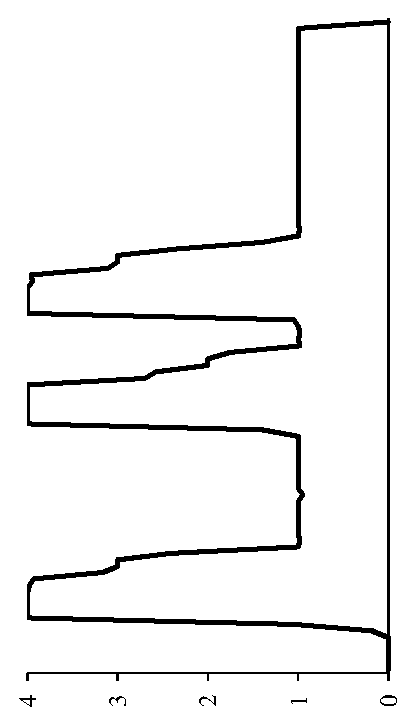
\includegraphics[scale=0.7,angle=270]{profile.eps}
\caption{Build parallelism.}
\label{fig:profile}
\end{figure}

\begin{figure}
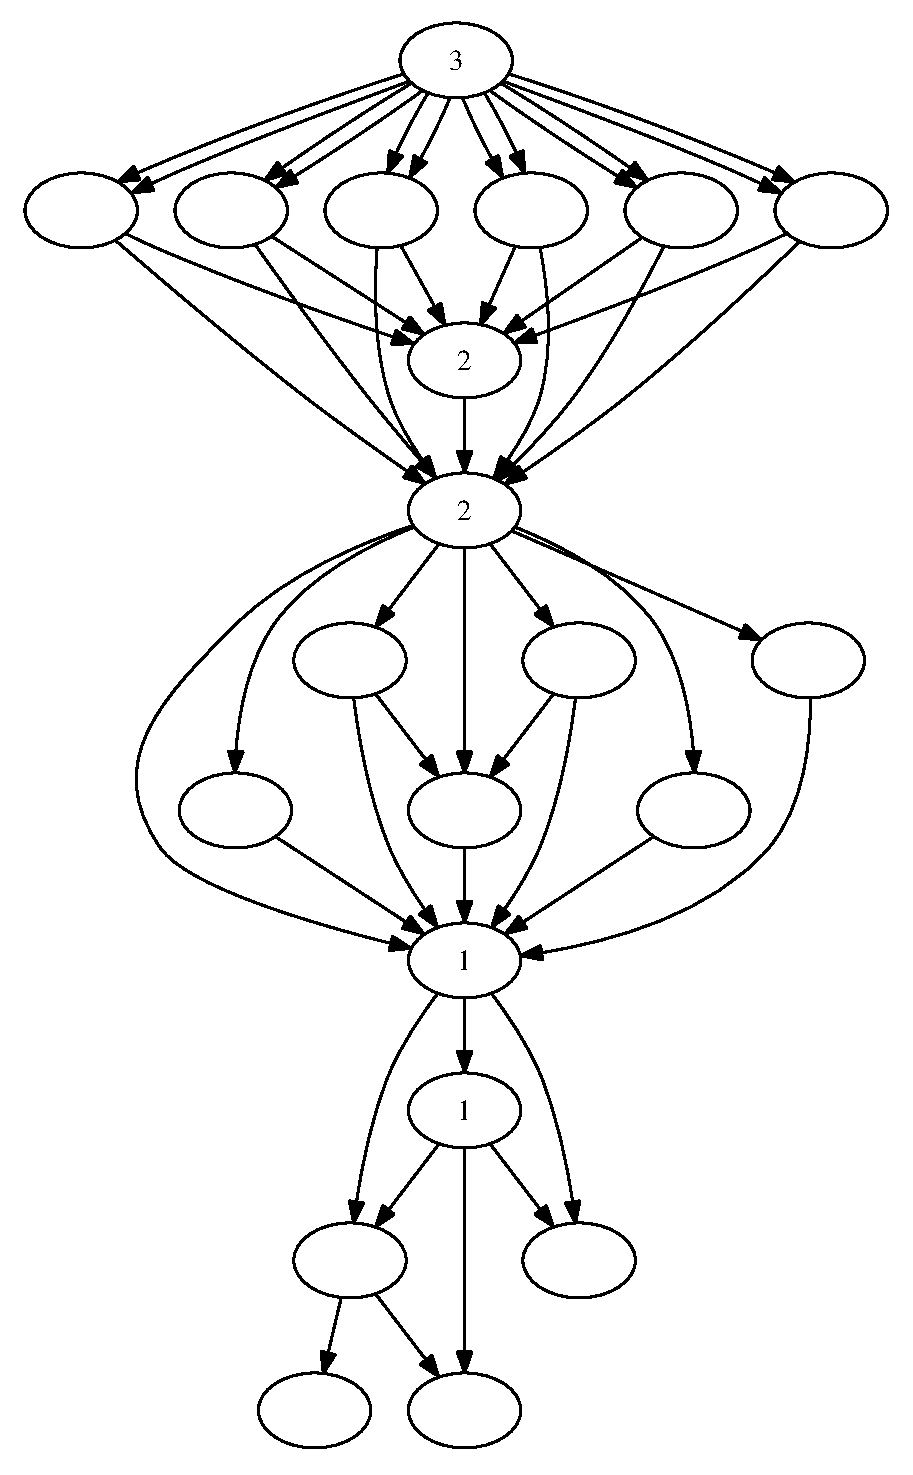
\includegraphics[scale=0.5]{layout.eps}
\caption{Dependency graph.}
\label{fig:analysis}
\end{figure}

% FINAL NUMBERS
% GHC full = 7.688
% GHC zero = 0.532
% Shake full -j1 = 11.828 (of which 11.702 is system commands)
% Shake full -j4 = 7.414 (of which 12.906 is system commands)
% Shake zero = 0.101 (of which 0.06 is ghc-pkg, 75% of the rest is writing the db)

As an example of the profiling and analysis tools in practice, see Figures \ref{fig:profile} and \ref{fig:analysis}. Both these diagrams are produced by building a 24 module Haskell program\footnote{The program is Shake itself, which can be compiled using Shake.} from scratch with a maximum of four processors. The entire process takes 7.41 seconds, but spends 12.91 seconds executing rules, giving a parallel speed up of 1.7 times. Executing the build system with one processor takes 11.83 seconds, where the reduced time compared to the rule execution time is likely due to reduced disk contention.

Figure \ref{fig:profile} shows the number of traced system commands executing at any point during the build. We see a start up period where zero commands are running and the build system is checking for dependencies, followed by three spikes up to four processors, followed by a tail of using one processor.

Turning to the dependency graph in Figure \ref{fig:analysis}, we have the |Main| module at the top labelled 3. This graph shows the dependencies of the \file{.hi} files, after hiding three leaf utility modules which are include in many places and have no dependencies (they add lots of lines, obscuring the real dependency graph). It is clear the build proceeds in three stages, with bottle-neck dependencies marked 1, 2 and 3. These three dependencies account for the three periods of one processor usage. The final tail of one processor includes both compilation of the main module (which profiling tells us takes 0.23 seconds) and linking (which takes 1.54 seconds).

This example shows how Shake's profiling and analysis reports can be used to improve build performance. If the bottle-neck modules could be split up, or if their compilation time was reduced (particularly for those marked 1, which account for a longer single processor section), the overall build speed would increase. In practice, we have found that for large build systems, where Shake is building multiple targets, the parallelism usually stays at the maximum (or fractionally below it) for most of the build time, before reducing down to one processor as the last few tasks complete.

\subsubsection{Comparison to @ghc --make@}

Building the same project with the GHC compilation system \cite{ghc7_2}, using \prog{ghc --make}, takes 7.69 seconds, compared to Shake with 11.83 seconds for one processor and 7.41 seconds for four processors. The reason GHC is quicker on one processor is that GHC keeps all interface information and package database information in memory, whereas running separate \prog{ghc -c} compilation commands requires reloading this information each time. However, Shake is able to use parallelism to improve the build time, while GHC cannot.

When running the build system while nothing needs compiling, GHC takes 0.54 seconds and Shake takes 0.10 seconds. Of the 0.10 seconds required by Shake, 0.06 seconds is spent checking the GHC installation has not changed (running @ghc-pkg list@) -- if the GHC installation is assumed to be constant Shake requires only 0.04 seconds. Shake is faster because it reads in one file (the database) then quickly checks |validStored| on a small number of files. GHC must at least query the same file information, but also has to construct a dependency graph, aggregating information from many files. Of that 0.4 seconds, 0.3 is spent writing the database -- we suspect that effort spent improving the binary serialisation would pay off.

% Compared to something like gcc, which is always invoked in single mode, we do better.
% For something like C# we don't have a choice and always run it in --make mode.

%if 0

\subsection{Lint checking}
\label{sec:lint}

\todo{write lint checking}

In order to remain consistent throughout the execution, we require that all externally stored values do \textit{not} change during the execution, other than as a result of running an |action| which |creates| it. The \make{} tool requires a similar property or it becomes inconsistent.

We end with a note of caution. We require that any stored value remains consistent other than when a rule actively changes in. Since this rule does not force the existence of a file, it should not be used on any files that may be generated by the build system -- |doesFileExist| should return the same at the start and end of the compilation. This property can be checked with Lint mode as described in \S\ref{sec:lint}.

Writing a large build system is a complex endeavour.

Can we roll it right back? Look which files a system command uses, and from that build the profiling report? Might work better on Windows.

It is never harmful to include an additional call to |need|, in fact, sometimes it is beneficial! Consider the following example:

\h{expr}\begin{code}
"file.txt" *> \out -> do
    need [out ++ ".part1", out ++ ".part2"]
    part1 <- readFile' (out ++ ".part1")
    part2 <- readFile' (out ++ ".part2")
    writeFile' out (part1++part2)
\end{code}

Here we use the additional function |writeFile'|, simply |writeFile| lifted to the |Action| monad. This rule would work correctly without the |need| call on the second line, as both |readFile'| calls include |need| within them. However, when running the build system in parallel, the additional |need| allows both dependencies to be computed at the same time, while the |need| calls inside |readFile'| serialise building of the dependencies.


There are two primary things we check for with lint. To get a full build we build everything, run whatever clean action the user has specified, then rerun each rule. The best lint will come if you:

* clean everything, apart from the database
* build with --lint

It's important when rebuilding to require the rules bottom up, i.e. the want statements should be replaced with something doing a bottom up traversal.

lint with invariants can always be done very easily.

lint with observations is much harder, since you don't want observations to overlap. that means you have to run the rules bottom up. or can try and subtract rules?

\subsubsection{Invariant information}

Things like whether a file exists or not should be constant throughout, otherwise any files which don't know will get confused. This can be checked by cleaning, and then running. Any key that marks itself as invariant should not change during this process. To do so, we add to the |Rule| class:

\begin{code}
invariant :: key -> Bool
invariant _ = False
\end{code}

\subsubsection{Dependency creation}

When running a file we can ask what has been changed, and what has been used. When we run just a rule, but no dependencies, the list of things that change must all be things who had rules run on them, and the list of things that were used should be equivalent.

\begin{code}
data Observed alpha = Observed {created :: Maybe [alpha], used :: Maybe [alpha]}

observed :: IO alpha -> IO (Observed key, alpha)
observed act = do res <- act; return (Observed Nothing Nothing, res)
\end{code}

Note that our original design simply passed an \h{type}|IO ()| to observed, and required the function to execute it. Alas, this went wrong since it's too easy to write an incorrect version that fails to execute! Now, thanks to parametricity, if you don't pass an error back, you must have got it right!

Given a set of observations, we can check what a key used in its body, and what it declared to create. However, there are a number of situations where people don't write 100\% accurate dependencies, but the effect is equivalent. For example, assuming \file{temporary.txt} is unused in the result of the build system, the following two rules seem morally equivalent:

\h{do}\begin{code}
"foo.txt" *> \out -> copyFile' "bar.txt" out

"foo.txt" *> \_ -> need ["temporary.txt"]
"temporary.txt" *> \out -> do
    copyFile' "bar.txt" "foo.txt"
    writeFileLines "temporary.txt" []
\end{code}

We can imagine more complex examples, and do define such examples in \ref{sec:multiple_outputs}. Therefore, we require the following properties:

\begin{itemize}
\item If you create a key that someone else requires, you must be a dependency of them.
\item If you use a key, you must depend on that key directly.
\item If you use a key but do not require it, you are safe, but conservative.
\end{itemize}

%endif

\section{Related Work}
\label{sec:related_work}

Build systems can be divided into two categories -- those which target single-language projects with fixed rules (e.g. \prog{ocamlbuild}, \prog{ghc --make}, Visual Studio projects), and those which are more general allowing user specified rules (e.g. \make{} and Shake). Focusing on the second category, the defacto standard is \make{}, but there are many \make{} competitors (notably Ant, CMake, Jam, Scons and Waf). Most of these tools read a rule list, generate a dependency graph, then execute commands while traversing that graph.

Since the number of build systems is vast, we have focused on four build systems which take different approaches (Redo, Ninja, Fabricate and Tup). Interestingly, the main thing all four systems have in common is that they require some external database of build data, in addition to the rules and file system. Unlike Shake, all these build systems are strictly limited to files.

\subsection{Redo}

% https://github.com/apenwarr/redo

The Redo build system \cite{redo} is certainly the most similar to Shake in its underlying theory. Rules are run starting at the target. A rule may call \ignore|redo-ifchange| (similar to |need|) to ensure that this rule is repeated if any of the file arguments change. Rules can be specified to build either a specific named file, or a set of files ending with a particular extension -- more precise rules can be implemented by defining a single rule with different behaviors based on the output filename.

While Redo is similar to Shake in theory, the practical implementation is significantly different, resulting in different levels of power. Instead of having a single rule store, Redo stores each rule in a separate file, and the script language is simply shell script, where \ignore|redo-ifchange| is a program. The advantage of separate files is that Redo is able to depend on the actual rule to build the output, meaning if the build system changes the correct and minimal build elements will be rebuilt. However, separating each build rule makes it harder to reason about the build system, and eliminates many potential uses of abstraction \cite{jonge:build_components}. Redo does not support unchanging files, doesn't work on Windows, and has no support for multiple outputs.

\subsection{Ninja}

% http://martine.github.com/ninja/manual.html

The Ninja build system \cite{ninja} is designed as a two-stage build system -- users specify their build rules in some high-level manner, which is then translated to a set of Ninja build rules. As a result, the Ninja build system is not designed to be general purpose and configuration choices are expected to be resolved by the first level. The Ninja target language supports three dependency features beyond \make{}. Firstly, a rule can depend on the list of files contained in another file, allowing dynamic dependencies. Secondly, the command line for each rule is tracked, resulting in a rebuild if the rule itself changes. Thirdly, a rule can generate multiple outputs, which are properly tracked.

\subsection{Tup}

% http://gittup.org/tup/build_system_rules_and_algorithms.pdf

The Tup build system \cite{tup} is designed as an incremental build system. Tup has a similar dependency structure to \make{}, but has a significantly different implementation. Instead of scanning all dependencies, it expects the operating system to supply a list of changed files, avoiding the overhead of checking which files have changed. For large build systems the result can be a significant speed improvement for builds with few files to rebuild. We believe a similar implementation strategy could be applied to Shake, also turning it into an incremental system.

Another significant difference in Tup is the automatic treatment of dead build objects. If a rule to build \file{foo} is deleted from the rule list, then Tup automatically deletes the file \file{foo}. The problem of old build objects can be serious, resulting in builds succeeding that should have failed, and that will fail as soon as a clean build is performed (to alleviate this risk, we use an overnight build which starts from scratch). However, we have a configuration which generates a basic IDE project file, which is then modified by the user -- deleting that file after the build rule disappears would be most unwelcome. We could add support for deleting dead build objects to Shake, but chose not to.

\subsection{Fabricate}

% http://code.google.com/p/fabricate/

The key innovation in the Fabricate build system \cite{fabricate} is that dependencies do not need to be given explicitly. A build system is described as a Python program, which primarily executes system commands in order. While executing the commands, Fabricate uses system tracing (strace on Linux) to record which files are accessed. In future runs, if the same system command is reached but none of its required files have changed, the command is skipped. The resulting build systems are simple, and avoid the difficulties of correctly specifying dependencies.

There are two inherent difficulties for designing a build system without explicit dependencies. Firstly, the system tracing mechanisms on different platforms are varied, and in particular on Windows are somewhat fragile, requiring hooking system libraries or checking for last-access times. Secondly, parallelism needs to be expressed manually -- Fabricate requires the addition of explicit grouping annotations before parallelism can be used.

\subsection{Haskell Build Libraries}

There are a surprising number of Haskell libraries implementing a full dependency based build system -- we are aware of ten excluding Shake (Abba, Blueprint, Coadjute, Cake, Cake\footnote{There are two distinct build libraries for Haskell named Cake!}, Hake, Hmk, Nemesis, OpenShake and Zoom). Of these, the two Cake libraries and OpenShake are derived from an early presentation of the principles behind Shake, before the source code was available. The primary difference from the Cake libraries is that Shake as presented in this paper allows multiple different types of build rule, while the Cake libraries only allow file rules. Compared to OpenShake \cite{openshake}, we have opted to have |rule|/|apply| based on dynamic types, and then expect everyone to use sugared versions to regain static guarantees of type safety. In contrast, OpenShake uses type functions \cite{schrijvers:type_functions} to statically track the available rule types, reducing the complexity of serialisation (\S\ref{sec:dynamically_typed}), but increasing the complexity of the library -- but compared to the similarities, this differences are minor.

\section{Conclusions}
\label{sec:conclusions}

We have shown how the dependency specification mechanism in build tools can be generalised, allowing additional dependencies to be specified \textit{after} previous dependencies have been examined. We have implemented our ideas as the Haskell library Shake, which is used to compile tens of millions of lines of code every day. The Shake build tool is more powerful than \make{}, and eliminates many awkward workarounds that are often required when writing build systems, especially when generated files are used.

While our build library has been optimised, saving the database is a noticeable bottleneck when builds run few actions, taking 75\% of the time. We suspect this step could be sped up, perhaps by switching to a different binary serialisation library. We have provided some profiling and analysis tools, but more would certainly be welcome.

The \make{} tool has been ubiquitous for the last thirty years, specifying dependencies in advance and defining actions with shell scripting and a macro system. With Shake we offer more powerful dependencies, coupled with the Haskell language for defining actions. The dependencies allow more complex build systems to be specified in a more direct manner, while the use of Haskell allows abstraction and reuse. We hope these advantages are powerful enough to tempt many developers to consider Shake.

\subsection*{Acknowledgements}

Thanks to Standard Chartered, where Shake was initially developed. Thanks to Raphael Montelatici for the name Shake. Thanks to Max Bolingbroke and Evan Laforge for many discussions about Shake.


\bibliographystyle{plainnat}
\balance
\bibliography

\end{document}
